\subsection{Understanding 160 \& 80-Meter Antennas: Common Truths!}

\begin{tcolorbox}[colback=gray!10, colframe=black, title=E9H02] 

Which is generally true for 160- and 80-meter receiving antennas?
\begin{enumerate}[label=\Alph*)]
    \item \textbf{A.} Atmospheric noise is so high that directivity is much more important than losses
    \item B. They must be erected at least 1/2 wavelength above the ground to attain good directivity
    \item C. Low loss coax transmission line is essential for good performance
    \item D. All these choices are correct
\end{enumerate} \end{tcolorbox}



\subsubsection{Related Concepts}

In radio communication, especially within the amateur radio frequencies, understanding the characteristics of different frequency bands is crucial. The 160-meter (1.8-2.0 MHz) and 80-meter (3.5-4.0 MHz) bands are affected by various atmospheric conditions due to their lower frequencies. 

\subsubsection{Atmospheric Noise}
Atmospheric noise refers to the radio frequency interference caused by natural phenomena. It tends to be more pronounced at lower frequencies, such as those found in the 160 and 80-meter bands. Therefore, it is vital for operators in these bands to have antennas that can achieve significant directivity. Directivity helps in focusing on the desired signals while minimizing the reception of noise from unwanted directions.

\subsubsection{Antenna Height and Directivity}
While it is commonly suggested that antennas should be placed at least 1/2 wavelength above the ground to attain good directivity, this principle is particularly relevant for higher frequencies where ground reflections can affect signal quality. However, for 160 and 80 meters, the emphasis shifts towards managing atmospheric noise rather than strictly adhering to the height guidelines.

\subsubsection{Transmission Lines}
The choice of transmission line, whether it is low-loss coax or otherwise, is generally linked to performance issues experienced at higher frequencies. Although low-loss coax is beneficial, the greater concern in the context of 160 and 80 meters is dealing with atmospheric noise, making the statement in choice A more significantly related to the performance in these bands.

\subsubsection{Conclusion}
In summary, while all the statements offer insight into the requirements for effective operation on the 160 and 80-meter bands, atmospheric noise and the importance of directivity stand out as the most critical considerations for maximizing reception quality.

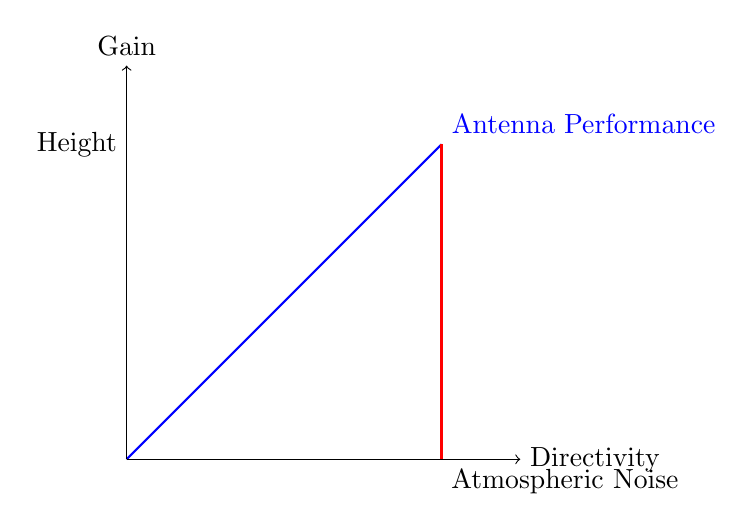
\begin{tikzpicture}[scale=1.0]
    \draw[->] (0,0) -- (5,0) node[right] {Directivity};
    \draw[->] (0,0) -- (0,5) node[above] {Gain};
    \draw[blue, thick] (0,0) -- (4,4) node[above right] {Antenna Performance};
    \draw[dashed] (0,0) -- (4,0) node[below right] {Atmospheric Noise};
    \draw[dashed] (0,0) -- (0,4) node[left] {Height};
    \draw[red, thick] (4,0) -- (4,4);
\end{tikzpicture}
